%% Testing paths with XeLaTeX
%% This gave me problems
\documentclass{article}
\usepackage{graphicx}
\usepackage{hyperref}
\usepackage{lipsum}
\ifxetex
  \usepackage{fontspec}
  \defaultfontfeatures{Mapping=tex-text}
  \usepackage{bera}
  %\setmainfont{fve}
  %\setsansfont{Myriad Pro}
  %\renewcommand{\ttdefault}{cmtt}
  %\setmonofont{Latin Modern Mono}
\else
  %\usepackage{lmodern}
  \usepackage{bera}
  \usepackage[T1]{fontenc}
\fi

\usepackage{algorithm2e} %lmodern,

%%\usepackage[toc,lof,lot]{multitoc}
\usepackage{fancyhdr}
%\usepackage{dateiliste}

\usepackage[listings,theorems]{tcolorbox}
\tcbset{before={\par\medskip\pagebreak[0]\noindent},after={\par\medskip}}%
%\usepackage{multicol}
\def\AmSmath{AmSmath}
%
\usepackage[main=english]{babel}
\usepackage{datetime} %%scrtime
\usepackage{xkvview}
\usepackage{hyperref}
%% hyperdoc has a problem with tcolorboc documentation
%% macros.
%%\usepackage{hypdoc}
\hypersetup{pdftex,
  bookmarks,
  raiselinks,
  pageanchor,
  hyperindex=true,
  colorlinks,
  allcolors=theblue, 
  linktocpage,
  hyperfootnotes=true,
  breaklinks=true,
  anchorcolor= blue,
  filecolor=blue,
  hypertexnames=true,
  backref,
  backref=page,
  pagebackref=true,
  urlcolor= teal,
  linkcolor= teal,
  pdftitle={My Title},
  pdfauthor={Yiannis Lazarides},
  pdfsubject={The phd LaTeX package},
  pdfkeywords={LaTeX package management, document design}
 }
\begin{document}
\section{Testing graphicspath}

\graphicspath{{./images/}}
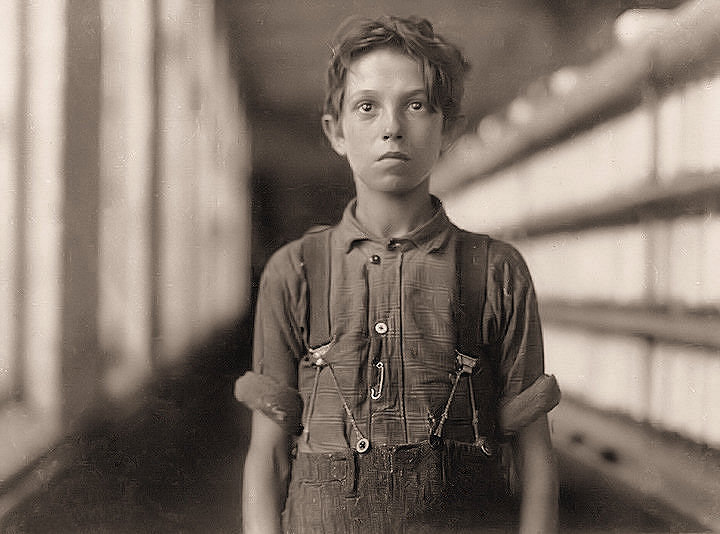
\includegraphics[width=0.5\textwidth]{hine02}

\lipsum[1]

\begin{verbatim}
\def\test{\@nil}
\end{verbatim}


\lstset{language={[LaTeX]TeX},
       escapeinside={{(*@}{@*)}}, 
       numbers=left, 
       gobble=0,
       stepnumber=1,numbersep=5pt, 
       numberstyle={\footnotesize\color{gray}},
       firstnumber=10,
       breaklines=true,
       framesep=5pt,
       basicstyle=\ttfamily,
       showstringspaces=false,
       stringstyle={\color{orange}\footnotesize},
       commentstyle=\color{orange!50},
       rulecolor=\color{black},
       breakatwhitespace=true,
       showspaces=false, 
       xleftmargin=10pt,
       xrightmargin=10pt,
       aboveskip=3pt plus1pt minus1pt, 
       belowskip=7pt plus1pt minus1pt,  
       backgroundcolor=\color{black!0.05}
}
\begin{lstlisting}{}

\lstset{language={[LaTeX]TeX},
       numbers=right, 
       gobble=0,
       stepnumber=1,numbersep=5pt, 
       numberstyle={\footnotesize\color{gray}},
       firstnumber=10,
       breaklines=true,
       framesep=5pt,
       basicstyle=\ttfamily,
       showstringspaces=true,
       stringstyle={\color{orange}\footnotesize},
       commentstyle=\color{orange!50},
       rulecolor=\color{black},
       breakatwhitespace=true,
       showspaces=false, 
       xleftmargin=10pt,
       xrightmargin=10pt,
       aboveskip=3pt plus1pt minus1pt, 
       belowskip=7pt plus1pt minus1pt,  
       backgroundcolor=\color{black!0.05}
}
%the string
\end{lstlisting}

\ifx\fmtname\nameofplainTeX
    true
\else
   false
\fi



\end{document}